\chapter{Analysis II}

\section{Potenzreihen}
Wir haben bis jetzt unter anderem die Grundlagen für Folgen und Reihen behandeln können und haben viele einige Funktionen wie z.B. $\exp$, $\sin$ und $\cos$ gesehen, welche wir durch Potenzreihen (je nach dem beliebig genau) approximieren konnten (i.e. Taylorapproximation). Wir können das ganze aber auch umdrehen und aus Potenzreihen ''neue'' Funktionen definieren.

Wir wollen nun also Funktionen betrachten, welche von folgender Form sind:
\begin{align}\label{eq_fcn_potenzreihe}
    f(x) = \sum^\infty_{n=0} a_n (x-a)^n
\end{align}
wobei die Koeffizienten $a_n \in \R$ oder $\C$ sind und $a \in \R$ den Entwicklungspunkt der Funktion bezeichnen soll. Überzeuge dich zuerst davon, dass diese Form von Potenzreihen die Allgemeinheit derer nicht einschränkt und für $a_0 = 0$ oder für $a = 0$ eindeutig ist.

Wir wollen uns nun zwei Fragen zu Potenzreihen stellen:
\begin{enumerate}
    \item Für welche $x$ konvergiert $f$?
    \item Was sind die Eigenschaften (Stetigkeit, Periodizität, Verhalten im Unendlichen, etc.) von $f$?
\end{enumerate}
Wie wir bereits erkannt haben, müssen Reihen, aus welchen Potenzreihen effektiv auch bestehen, nicht immer konvergieren. Da diese Reihen im Fall von Potenzreihen vom Argument $x$ abhängig sind, müssen wir für jedes $x$ entscheiden, ob die Potenzreihe konvergiert, i.e. ob die Potenzreihe einen eindeutigen Wert zurückgibt, i.e. was der Definitionsbereich von der Potenzreihe ist. Wir werden sehen, dass Potenzreihen in einem Bereich $-R < x-a < R$ also $|x-a| < R$ absolut konvergieren\footnote{Die Reihe (i.e. partielle Summen) der einzelnen Terme konvergiert.}. Wir nennen $R$ dann auch den \textbf{Konvergenzradius} und werden sehen, dass dieser durch den $\limsup$ konstruiert wird.

\subsection{Einschub: Der Limes superior}
Bis jetzt haben wir keine grossen Aussagen zu Folgen wie z.B. 
\begin{align}\label{eq_examble_limsup}
    (c_n)_{n=0}^\infty = (1.1, -0.9, 1.01, -0.99, 1.001, -0.999, 1.0001, ...)
\end{align} gemacht, ausser dass sie begrenzt sind aber trotzdem nicht konvergieren (i.e. divergieren?). Wir sehen aber trotzdem, dass eine Teilfolge nach $1$ und eine andere nach $-1$ konvergiert und im Limit auf den Bereich $[-1, 1]$ begrenzt sein wird. Hierfür wollen wir nun den Begriff des \textbf{Limes superior} $\limsup$ und des \textbf{Limes inferior} $\liminf$ einführen. Dabei betrachten wir für ein $n$ jeweils das Supremum (resp. Infimum) der Folgeglieder von $n$ (also den ''Rest'' der Folge ohne den ersten $n$ Elementen). Wir bilden aus den Suprema eine Folge und nehmen davon den Grenzwert.

\begin{definition}{Limes superior}{}
Sei $(c_n)_{n=0}^\infty$ eine beschränkte Folge in $\R$. Der \textbf{Limes superior} dieser Folge ist
$$\limsup_{n \to \infty}{c_n} = \lim_{n \to \infty}{\big(\sup\{c_k\mid k\geq n\}\big)}$$
\end{definition}

Wir können zeigen, dass \textit{jede} beschränkte Folge ein solches $\limsup$ besitzt: Betrachten wir die Mengen der Folgeglieder eines bestimmten Indexes $S_n = \{c_k \mid k \geq n\}$, welche einerseits nicht-leer und beschränkt sein muss. Aus der Konstruktion gilt nun:
$$S_1 \supseteq S_2 \supseteq S_3 \supseteq ... \implies \sup S_1 \geq \sup S_2 \geq \sup S_3 \geq ...$$
Da $(\sup S_n)_{n=0}^\infty$ eine monoton fallende, beschränkte Folge ist, erkennen wir durch
$$\limsup_{n \to \infty}  S_n = \lim_{n \to \infty} (\sup S_n) = \inf((\sup S_n)_{n=0}^{\infty})$$
dass der $\limsup$ existiert.

Analog ist der \textit{Limes inferior} definiert, jedoch können wir auch die Folge negieren und davon den $\limsup$ nehmen:
\begin{definition}{Limes inferior}{}
$$\liminf_{n \to \infty}{c_n} = -\limsup_{n \to \infty}{-c_n}$$
\end{definition}

\begin{example}In unserem Beispiel von vorher (\ref{eq_examble_limsup}) gilt somit $\limsup_{n \to \infty} c_n = 1$ und $\liminf_{n \to \infty} c_n = -1$
\end{example}

\begin{lemma}{Folgerungen}{limsup_consequences}
Sei $c_{n \to \infty}$ eine beschränkte Folge in $\R$. Folgende Aussage über $c \in \R$ sind äquivalent:
\begin{enumerate}
    \item Der $\limsup_{n \to \infty} c_n$ existiert
    \item \begin{enumerate}
        \item \textit{(Obere Grenze)} Falls für ein $a \in \R: a > c$ gilt, dann gilt für alle (ausser endlich viele) Nachfolgerelemente $c_n < a$.
        \item \textit{(Untere Grenze)} Falls für ein $b \in \R: b < c$ gilt, dann gilt für unendlich viele Nachfolgerelemente $c_n > b$
    \end{enumerate}
\end{enumerate}
\end{lemma}
In Worte gefasst: Da $c$ der $\limsup$ von $c_{n \to \infty}$ ist, gibt es Teilfolgen, welche nach $c$ konvergieren. Nun haben wir ein $a > c$; man kann es sich als $c + \varepsilon$ vorstellen. Da wir aus der Definition wissen, dass es über $c$ zu keiner Konvergenz kommen kann, müssen alle Glieder sich ab einem bestimmten $n$ im Streifen unter $a$ befinden. Für das $b<c$, welches wir uns als $c - \varepsilon$ vorstellen können, kann man dieselbe Aussage im Allgemeinen nicht mehr machen. Da es aber Teilfolgen gibt, die nach $c$ konvergieren, müssen sicher unendlich viele Glieder grösser als $b$ sein. 

\begin{proof} (1. $\Longrightarrow$ 2.) ist als Übung zu lösen (Lösung im Skript Abschnitt 5.2.2)

(2. $\Longrightarrow$ 1.): Seien $a > c > b$, wähle $\varepsilon_a = 2(a - c) > 0$ und $\varepsilon_b = c - b > 0$.
\begin{enumerate}[label=(\alph*)]
    \item Es existiert ein $n_0$ gibt, sodass für alle Suprema der darauf folgenden Glieder kleinergleich\footnote{wegen der Definition des Supremums} $c + \frac{\varepsilon_a}{2}$ gilt, also:  $\sup \{c_k \mid k \geq n\} \leq c + \frac{\varepsilon_a}{2}$ mit $n \geq n_0$. Wir erhalten somit: $\sup \{c_k \mid k \geq n\} \leq c + \frac{\varepsilon_a}{2} < c + \varepsilon_a < a$.
    \item Da $c$ ein Konvergenzpunkt von Teilfolgen ist, gibt es für jedes $n$ ein $k \geq n$, sodass $c_k > c - \varepsilon_b = b$ gilt. Das impliziert $\sup \{c_k \mid k \geq n \}> c - \varepsilon = b$
\end{enumerate}
Sei nun $\varepsilon = \min\{\varepsilon_a, \varepsilon_b\}$, dann gilt $c-\varepsilon < \sup\{c_k \mid k \geq n\} < c+\varepsilon$ für $n \geq n_0$. Lassen wir $n$ nun nach Unendlich laufen, erhalten wir die Behauptung:
$$\lim_{n \to \infty}{\sup \{c_k \mid k \geq n\}} = c$$
\end{proof}

\begin{remark}
\begin{enumerate}
    \item Falls nun die gesamte Folge $(c_n)$ konvergiert, dann gibt es zu jedem $\varepsilon >0$ ein $n_0$ so dass $c-\varepsilon < c < c + \varepsilon$, also a) und b) gelten. Daraus folgt $\limsup_{n \to \infty} c_n = \lim_{n \to \infty} c_n$
    \item Aus dem Lemma folgt, dass im Allgemeinen $c = \limsup_{n \to \infty} c_n$ der grösste Häufungspunkt (also der grösste Grenzwert aller konvergierenden Teilfolgen von $(c_n)_{n=0}^\infty$)
    \item Analog gelten alle Eigenschaften auch für das Infimum: $\liminf{c_n} = -\limsup{-c_n}$
    \item Es gilt eine (auf positive Werte begrenzte) Homogenität: $\limsup{\lambda c_n} = \lambda \limsup{c_n}$ für $\lambda \in \R_{>0}$
\end{enumerate}
\end{remark}

Zu guter Letzt verwenden wir für nicht von oben beschränkte Folgen $(c_n)_{n=0}^\infty$ die Konvention
$$\limsup_{n \to \infty} c_n = \infty$$
In diesem Fall gilt 2b) aus obigem Lemma für alle $b \in \R$.

\subsection{Einschub: Wurzelkriterium und Limes Superior}
Nun nochmal einen kurzen Theorieeinschub um die Brücke zwischen dem soeben definierten $\limsup$ und dem \textsc{Cauchy}-Wurzelkriterium zu schlagen. Hier nochmals das Wurzelkriterium zur Erinnerung:

Sei $(c_n)_{n=0}^\infty$ eine Folge in $\R$ oder $\C$:
\begin{enumerate}
    \item Falls $\sqrt[n]{|c_n|} < 1$ für alle (ausser endlich) viele $n$ gilt, dann konvergiert die Reihe von $(c_n)_{n=0}^\infty$ absolut, d.h. die Summe der Absolutbeträge $\sum_{n=0}^{\infty}|c_n|$ konvergiert.
    \item Falls $\sqrt[n]{|c_n|} > 1$ für unendlich viele $n$ gilt, divergiert die Reihe $\sum_{n=0}^{\infty}|c_n|$ (da $(c_n)_{n=0}^\infty$ keine Nullfolge ist.) Insbesondere konvergiert sie nicht absolut.
\end{enumerate}

Die Konvergenz der Reihe von einer Folge $(c_n)_{n=0}^\infty$ unter dem Wurzelkriterium besagt in Worten ausgedrückt, dass ''die Reihe von $(c_n)_{n=0}^\infty$ höchstens so schnell wächst wie die geometrische Reihe''.

\begin{satz}{Umformulierung des Wurzelkriteriums}{limsup_root_crit}
\begin{enumerate}
    \item Falls $\limsup_{n \to \infty} \sqrt[n]{|c_n|} < 1$ gilt, dann konvergiert $\sum_{n=0}^{\infty}|c_n|$
    \item Falls $\limsup_{n \to \infty} \sqrt[n]{|c_n|} > 1$ gilt, dann divergiert $\sum_{n=0}^{\infty}|c_n|$
\end{enumerate}
\end{satz}

\begin{remark}
Über $\limsup (...) = 1$ kann wie beim Wurzelkriterium keine Aussage gemacht werden
\end{remark}

\begin{proof}
Verwende obiges Lemma \ref{lem:limsup_consequences}. Für 1. wähle $a$, sodass $\sqrt[n]{|c_n|} < a < 1$ gilt. Für 2. wähle $b = 1$
\end{proof}

\subsection{Konvergenzverhalten}
Nun haben wir die nötigen Begriffe erarbeitet und können zu den Potenzreihen zurückkehren, von denen wir nun das Konvergenzverhalten bestimmen wollen. Wir werden die obige Form des \textsc{Cauchy}-Wurzelkriteriums verwenden, um den \textbf{Konvergenzradius} um $0$ herum zu bestimmen, d.h., dass wir vorerst den Entwicklungspunkt oder den ''Mittelpunkt'' $a = 0$ setzen. Die Behauptung zur Konvergenz von Potenzreihen ist folgende:

\begin{satz}{Konvergenzradius, Formel von Hadamard}{konvergenz_von_potreihen}
Sei $(a_n)_{n=0}^\infty$ eine Folge in $\R$ oder $\C$, dann gilt für den \textbf{Konvergenzradius} $R$ von $f(z) = \sum_{n=0}^\infty a_n z^n$:

$$R = \frac{1}{\limsup_{n \to \infty}\sqrt[n]{|a_n|}} \in [0, \infty]$$

d.h. für ein beliebiges $z \in \C$ die Reihe $\sum_{n=0}^\infty a_n z^n$ absolut genau dann, wenn $|z|< R$ gilt. Für $|z|>R$ divergiert die Reihe.
\end{satz}

\begin{remark} Auch hier können wir keine Aussage über das Konvergenzverhalten auf dem Rand machen. Dieses muss für Punkt des Kreises auf andere Weise berechnet werden.
\end{remark}

\begin{proof}
Wir wenden Satz \ref{satz:limsup_root_crit} an auf $c_n = a_nz^n$ und erhalten $\sqrt[n]{|c_n|} = \sqrt[n]{|a_nz^n|} = \sqrt[n]{|a_n|}\cdot|z|$. Wir erkennen, dass die Reihe immer konvergiert für $|z| = 0 = z$. Dies kann man auch intuitiv leicht am Polynom $f(0)$ erkennen: Alle Terme sind 0 ausser der konstante Term $a_0$, welcher endlich ist. Nun sei $|z| \neq 0$, dann muss für die Konvergenz mit dem Wurzelkriterium gelten:
$$\limsup_{n \to \infty} \sqrt[n]{|c_n|} = \limsup_{n \to \infty} \sqrt[n]{|a_nz^n|} \stackrel{Bem. 4.}{=} |z| \limsup_{n \to \infty} \sqrt[n]{|a_n|} < 1$$
Wir erhalten durch Umstellung den folgenden Ausdruck und definieren damit den Konvergenzradius:
$$|z| < \frac{1}{\limsup_{n \to \infty} \sqrt[n]{|a_n|}} =: R$$
Für die Konvergenz gilt also die Beziehung: $\limsup_{n \to \infty} \sqrt[n]{|c_n|} = \frac{|z|}{R} < 1$. Falls im anderen Fall also  $\frac{|z|}{R} > 1$ gilt, divergiert die Reihe.
\end{proof}

\begin{example} Hier einige Beispiele:
\begin{enumerate}[label=\alph*)]
    \item Exponentialfunktion $e^z = 1 + \sum_{n = 1}^\infty \frac{z^n}{n!}$. Das Supremum eines Elements $n$ ist jeweils $\frac{1}{n!}$, somit erhalten wir also für den Konvergenzradius:
    $$R = \frac{1}{\limsup_{n \to \infty}\sqrt[n]{\frac{1}{n!}}} = \frac{1}{\lim_{n \to \infty}\sqrt[n]{\frac{1}{n!}}} = \infty$$
    \item Geometrische Reihe $\sum_{n = 1}^\infty z^n = \frac{1}{1-z}$: Es folgt direkt, dass $R = 1$ gilt. Somit konvergiert es nur absolut für $|z| < 1$
    \item $\sum_{n = 1}^\infty n! z^n$: Die Reihe ist nicht begrenzt: $\lim_{n \to \infty} \sqrt[n]{|n!|} = \infty$, also ist das Supremum für alle $n$ gleich $\infty$ und somit gilt für den Limes Superior auch $\limsup_{n \to \infty}\sqrt[n]{|n!|} = \infty$. Es folgt $R =$ ''$\frac{1}{\infty}$'' $ = 0$. $z = 0$ nennen wir in diesen Fall einen \textbf{konvergenten Randpunkt}.
\end{enumerate}
\end{example}

Bis jetzt haben wir alles für Potenzreihen ''um den Ursprung'' mit $a = 0$ gezeigt. Wir wollen nun in einen letzten Schritt diesen Mittelpunkt um $a$ verschieben, um die Form aus (\ref{eq_fcn_potenzreihe} zu erhalten:

\begin{lemma}{}{}
Die Potenzreihe
$$\sum_{n = 1}^\infty a_n (x-a)^n$$
mit Mittelpunkt $a \in \R$ konvergiert absolut im Intervall $(a-R, a+R)$, wobei 
$$R = \frac{1}{\limsup_{n \to \infty}\sqrt[n]{|a_n|}} \in [0, \infty]$$
\end{lemma}

\begin{proof}
Hierfür setzen setzen wir $z = x - a$ in die obigen Definitionen ein.
\end{proof}

Der Konvergenzbereich ist also eine Kreisscheibe in $\C$ um $a$ mit Radius $R$. 

\subsection{Summen und Produkte von Potenzreihen}
Wir können des Weiteren auch Summen und Produkte zweier Potenzreihen bilden: Seien $\sum a_n z^z$ und $\sum b_n z^z$ zwei Potenzreihen mit Konvergenzradien $R_a$ und $R_b$, somit konvergieren beide für $z \in \C$ im Bereich $|z| < R$, wobei $R = \min\{R_a, R_b\}$ gilt. Es folgen also für Summen und Produkte:
\begin{align*}
    \sum_{n = 0}^\infty a_n z^n + \sum_{n = 0}^\infty b_n z^n &= \sum_{n = 0}^\infty (a_n + b_n) z^n\\
    (\sum_{n = 0}^\infty a_n z^n)(\sum_{n = 0}^\infty b_n z^n) &= \sum_{n = 0}^\infty (a_0b_n + a_1b_{n-1} + ... + a_nb_0 )z^n
\end{align*}
welche absolut konvergieren für $|z| < R$. Für die Multiplikation wurde das Cauchy-Produkt zweier absolut konvergenter Reihen verwendet.
$$*\ *\ *$$

Nun haben wir unsere erste Frage bezüglich der Konvergenz beantworten können. Um die zweite Frage zu den Eigenschaften von Potenzreihen zu beantworten wollen wir etwas ausholen:

Eine Potenzreihe sieht ja im Allgemeinen in etwa so aus:
$$f(x) = a_0 + a_1(x-a) + a_2(x-a)^2 + a_3(x-a)^3...$$
Der Funktionswert $f(x)$ ist also der Grenzwert der Reihe der einzelnen Terme oder anders ausgedrückt der Grenzwert aus der Folge der Partialsummen:
$$f(x) = \lim_{n \to \infty}\Big( \sum_{k=0}^n a_k(x-a)^k \Big)$$
Wir können daher also eine Funktion $f_n$ definieren, welche nur die ersten $n$ Terme von $f$ aufweist. Diese Funktion $f_n$ wird nur bis zu einem gewissen Grad Ähnlichkeiten mit $f$ haben, lässt man aber den Index $n$ nach $\infty$ laufen, so inkludieren wir immer mehr Terme von $f$, wobei wir im Limit (im Konvergenzbereich versteht sich) $\lim_{n \to \infty} f_n = f$ erhalten.

Wir könnten nun aber auch eine Folge von diesen Partialsummenfunktionen $f_n$ konstruieren, also $(f_1, f_2, f_3, ...)$. Werten wir alle Funktionen bei einem $x$ aus, so erhalten wir eine Folge in $\R$, dessen Grenzwert $f(x)$ sein muss. Wir können also Potenzreihen als Limit von Funktionenfolgen schreiben. Wir wollen also kurz allgemeine Eigenschaften von solchen Funktionenfolgen zeigen:

\subsection{Einschub: Konvergenz von Funktionenfolgen}\label{cha_funktionenfolgen}
Wir wollen also eine Folge konstruieren, dessen Elemente Funktionen sind: $(f_1, f_2, f_3, ...)$. Sie sollen alle den selben Definition- und Wertebereich besitzen, wir verwenden $f_i: D \to \R$, wobei $D \subseteq \R$ eine nicht-leere Teilmenge von $\R$ ist. Im Allgemeinen sind alles verschiedene Funktionen, im Fall von Partialsummen von Potenzreihen jedoch unterscheiden sie sich nur in der vom Index $i \in \N$ abhängigen Länge.

Diese Folge von Funktionen liefert für jedes Argument $x \in D$ eine ''normale'' Folge in $\R$: $(f_1(x), f_2(x), f_3(x), ...)$, somit können wir sie und die daraus entstehenden Reihen auf Konvergenz untersuchen und erhalten daraus je nach dem einen Grenzwert. Macht man das nun für alle $x \in D$, so erhält man quasi eine ''Grenzfunktion'' $f$, welche ausgewertet bei einem $x$ den Grenzwert der Folge von $\sum_{i=1}^\infty f_n(x)$ gibt. Hierzu wollen wir nun zwei Begriffe der Konvergenz definieren:

\begin{definition}{Punktweise Konvergenz}{}
Sei $D \subseteq \R, D \neq \emptyset$. Die Folge $(f_n:D \to \R)^\infty_{n=0}$ \textbf{konvergiert punktweise} [pointwise] gegen $f: D \to \R$ falls
$$\lim_{n \to \infty} f_n(x) = f(x)$$
für alle $x \in D$.
\end{definition}

\begin{definition}{Gleichmässige Konvergenz}{}
Sei $D \subseteq \R, D \neq \emptyset$. Die Folge $(f_n:D \to \R)^\infty_{n=0}$ \textbf{konvergiert gleichmässig} [uniformly] gegen $f: D \to \R$, falls zu jedem $\varepsilon >0$ ein Index $n_0$ existiert, sodass:
$$\forall n\geq n_0: |f_n(x) - f(x)| < \varepsilon $$
für alle $x \in D$ gilt.
\end{definition}
\begin{remark}
Die Definitionen sind sehr ähnlich, beachte aber die Reihenfolge der Quantoren: Für die punktweise Konvergenz betrachten wir zuerst ein $x$ und wählen dann das passende $n$, sodass $|f_n(x)-f(x)| < \varepsilon$ (kommt aus der Definition des Limes). Bei der gleichmässigen Stetigkeit hingegen soll das $n_0$ --- nach der Wahl eines $\varepsilon$ --- für alle $x \in D$ gelten. Also darf das $n_0$ nur von $\varepsilon$ abhängen, nicht aber von $x$. Somit ist die gleichmässige Konvergenz einschränkender und die punktweise Konvergenz folgt aus der gleichmässigen Konvergenz.
\end{remark}

\begin{example}\label{ex_grenzfunktion} Wir definieren die Funktionenfolge wie folgt:

\begin{minipage}[c]{0.4\linewidth}
$$f_n: D=[0,1] \to \R$$
$$x \mapsto \begin{cases} 0 & x >\frac{1}{n} \\ 1-nx & x \leq \frac{1}{n}\end{cases}$$\\
\end{minipage}
\hspace{2em}
\begin{minipage}[]{0.4\linewidth}
\begin{tikzpicture}
    \begin{axis}[
        axis lines = left,
        xlabel = $x$,
        ylabel = {$f_n(x)$},
        xtick={0, 0.125,0.25,1},
        xticklabels={$0$,$\frac{1}{2n}$,$\frac{1}{n}$,$1$},
        ytick={0,0.5, 1},
        yticklabels={$0$,$\frac{1}{2}$,$1$},
        width=7cm,height=4cm,
    ]
    \addplot [domain=0:0.25, samples=5, color=red, style={thick}] {1 - 4*x};
    \addplot [domain=0.25:1, samples=5, color=red, style={thick}] {0};
    \addplot[mark=*, color=red] coordinates {(0.125,0.5)};
    \end{axis}
\end{tikzpicture}
\end{minipage}\hfill

Der punktweise Grenzwert dieser Funktionenfolge ist:
$$ \lim_{n \to \infty} f_n(x) = f(x) = \begin{cases} 0 & x >0 \\ 1 & x = 0\end{cases}$$
Wir erkennen zudem auch, dass diese Funktionenfolge nicht gleichmässig konvergiert, da es z.B. für $\varepsilon = \frac{1}{2}$ kein $n_0$ gibt, sodass für alle $x > 0$ die Bedingung $|f_{n_0}(x)-f(x)| < \varepsilon$ gilt. Betrachte hierfür z.B. den Punkt bei $\frac{1}{2n_0}$, welcher für jedes beliebig grosse $n_0$ stets eine Differenz von $\frac{1}{2}$ zu $f(\frac{1}{2n}) = 0$ aufweist.
\end{example}

\subsection{Folgerungen der gleichmässigen Konvergenz}

Die gleichmässige Konvergenz ist speziell, da einige Eigenschaften der Funktionen $f_n$ der Funktionenfolge an die Grenzfunktion ''weitervererbt'' werden können:

So gilt für die Grenzfunktion $f$ von Funktionenfolgen, bei der alle (ausser endlich viele) Elemente/Funktionen $f_n$ stetig sind, ebenfalls die Stetigkeit\footnote{Da wir jetzt von zwei verschiedenen ähnlichen Eigenschaften reden, muss man sich immer im Klaren sein, was nun konvergiert/stetig ist. Die Elemente $f_n(x)$ der Funktionenfolge sind für ein $x$ im Konvergenzradius absolut konvergent. Das sagt aber nichts über die Stetigkeit der Grenzfunktion $f$ aus, ausser dass sie dort definiert ist. Wie wir gesehen haben, kann diese trotz stetiger $f_n$ wie in obigem Beispiel \ref{ex_grenzfunktion} selber nicht stetig ist.}. Wir wollen also folgenden Satz zeigen:

\begin{satz}{Stetigkeit von Grenzfunktion}{stetigkeit_grenzfcn}
Ist $f_n: D \to \R$ (oder $\C$) eine Folge stetiger Funktionen auf $D \subseteq \R$ oder $\C$, die gleichmässig gegen die Funktion $f: D\to \R$ konvergieren, dann ist die Grenzfunktion $f$ stetig.
\end{satz}

\begin{proof} Sei $a \in D \subseteq \R, \varepsilon > 0$. Wir wollen zeigen, dass ein $\delta > 0$ existiert, sodass
$$\abs{x-a} < \delta \implies \abs{f(x) - f(a)} < \varepsilon$$
Wegen der gleichmässigen Konvergenz gibt es also ein $n_0$, sodass
$$\abs{f(x)-f_{n_0}(x)}<\frac{\varepsilon}{3}$$
gilt für alle $x\in D$. Aus der Stetigkeit von $f_{n_0}$ wissen wir zudem, dass es ein $\delta$ gibt, sodass 
$$\abs{f_{n_0}(x)-f_{n_0}(a)} < \frac{\varepsilon}{3}$$
gilt für $\abs{x-a} < \delta$. Nun formen wir den zu zeigenden Ausdruck mit der Dreiecksungleichung um, sodass wir die uns bekannten Ausdrücke erhalten:
\begin{align*}
    \abs{f(x) - f(a)} &= \abs{f(x) - f_{n_0}(x) + f_{n_0}(x) - f_{n_0}(a)+f_{n_0}(a) - f(a)}\\
    &\leq \abs{f(x) - f_{n_0}(x)} + \abs{f_{n_0}(x) - f_{n_0}(a)} + \abs{f_{n_0}(a) - f(a)}\\
    &< \frac{\varepsilon}{3} +  \frac{\varepsilon}{3} + \frac{\varepsilon}{3} = \varepsilon
\end{align*}
falls $\abs{x - a} < \delta$ gilt. Das zeigt also die Behauptung, dass wir eine stetige Grenzfunktion aus einer gleichmässig stetigen Funktionenfolge erhalten.
\end{proof}

Eine andere Eigenschaft, die die Grenzfunktion $f$ mit der gleichmässigen Konvergenz aus den Funktionen $f_n$ der Funktionenfolge ''erbt'', ist die \textsc{Riemann}-Integrierbarkeit\footnote{Erinnerung \textsc{Riemann}-Integrierbarkeit: $f:{a,b} \to \R$ ist \textsc{Riemann}-integrierbar genau dann, wenn es zu jedem $\varepsilon > 0$ Treppenfunktionen $u,o$ gibt mit $u \leq f \leq o$ und $\int_a^b(o-u)(x)dx < \varepsilon$}:

\begin{satz}{\textsc{Riemann}-Integrierbarkeit von Grenzfunktion}{fcnfolge_riem_inbarkeit}
Sei $a < b \in R$. Falls $f_n:[a,b] \to \R$ eine Folge aus \textsc{Riemann}-integrierbaren Funktionen ist, die gleichmässig gegen $f[a,b] \to \R$ konvergiert, dann ist $f$ Riemann-integrierbar und es gilt:
$$\lim_{n \to \infty} \int_a^b{f_n(x)}dx =  \int_a^b \lim_{n \to \infty}{f_n(x)}dx = \int_a^b {f_n(x)}dx$$
\end{satz}
Es wird also in anderen Worten behauptet, dass die Vertauschung des Limes-Operators und des Integrals erlaubt ist.

\begin{proof} (Teil I: \textsc{Riemann}-Integrierbarkeit) Die Beweisidee ist, ein $f_n$ zu finden, damit man aus deren (obere und untere) Treppenfunktionen entsprechende Treppenfunktionen für $f$ konstruieren können:

Wir legen im ersten Schritt einen $\tilde{\varepsilon}$-''Schlauch'' um $f$ (Das entspricht also der Fläche zwischen $f-\tilde{\varepsilon}$ und $f+\tilde{\varepsilon}$). Nun wollen wir ein $n$ finden, sodass $f_n$ ganz in diesem Schlauch liegt: Es soll also $f-\tilde{\varepsilon} < f_n(x) < f+\tilde{\varepsilon}$ resp. $\abs{f_n(x) - f(x)} < \tilde{\varepsilon}$ für alle $x \in [a,b]$ gelten.

Dann können wir wegen der \textsc{Riemann}-Integrierbarkeit von $f_n$ eine obere und eine untere Treppenfunktion $o_n$ und $u_n$ von $f_n$ finden, für welche $\int_a^b o_n(x) - u_n(x) dx < \tilde{\varepsilon}$ gilt. Da für $o_n$ und $u_n$ per Definition $u_n \leq f_n \leq o_n$ gilt und die Differenz zwischen $f_n$ und $f$ kleiner als $\tilde{\varepsilon}$ ist, können wir folgenden Ausdruck herleiten:
$$\underbrace{u_n(x) - \tilde{\varepsilon}}_{\tilde{u}_n(x)} \leq f_n(x) - \tilde{\varepsilon} < f(x) < f_n(x) + \tilde{\varepsilon} \leq \underbrace{o_n(x) + \tilde{\varepsilon}}_{\tilde{o}_n(x)}$$
Somit haben wir eine obere und eine untere Treppenfunktion für $f$ konstruieren können:
$$\tilde{u}_n(x) \stackrel{(<)}{\leq} f(x) \stackrel{(<)}{\leq} \tilde{o}_n(x)$$
Integriert man nun die Differenz von $\tilde{u}_n(x)$ und $\tilde{o}_n(x)$, so erhält man:
\begin{align*}
    \int_a^b(\tilde{u}_n(x)-\tilde{o}_n(x))dx &= \int_a^b(o_n(x) + \tilde{\varepsilon} - u_n(x) + \tilde{\varepsilon})dx\\
    &=\int_a^b(o_n(x) - u_n(x))dx + 2\tilde{\varepsilon}(b-a)\\
    &<\tilde{\varepsilon}+ 2\tilde{\varepsilon}(b-a)
\end{align*}
Nun können wir $\tilde{\varepsilon} = \frac{\varepsilon}{1+2b-2a}$ wählen, wodurch wir die \textsc{Riemann}-Integrierbarkeit von $f$ zeigen:
$$\forall \varepsilon > 0: \exists \tilde{u}_n, \tilde{o}_n: \Big(\tilde{u}_n \leq f \leq \tilde{o}_n\Big) \land \Big(\int_a^b(\tilde{u}_n - \tilde{o}_n)(x)dx < \varepsilon\Big)$$

(Teil II: Gleicher Grenzwert) Nachdem wir die Integrabilität gezeigt haben, wollen wir noch zeigen, dass das Integral von $f$ auch den selben Wert annimmt wie der vom Limit der Funktionenfolge. Wir wollen also zeigen, dass für ein $\varepsilon>0$
$$\abs{\int_a^b f_n(x) dx - \int_a^b f(x) dx} < \varepsilon$$
gilt. Ähnlich wie vorher (nur direkter ohne $\tilde{\varepsilon}$) können wir wegen der gleichmässigen Konvergenz $n$ wie folgt wählen:
$$\abs{f_n(x) - f(x)}<\frac{\varepsilon}{b-a}$$
Wir erhalten also für die Differenz der Integrale:
\begin{align*}
    \abs{\int_a^b f_n(x) dx - \int_a^b f(x) dx} &= \abs{\int_a^b f_n(x) - f(x) dx}\\
    &\leq \int_a^b \abs{f_n(x)- f(x)} dx\\
    &<\int_a^b \frac{\varepsilon}{b-a}dx\\
    &< \varepsilon
\end{align*}
Somit haben wir die Gleichheit der Integrale gezeigt, woraus die Behauptung folgt.
\end{proof}

\subsection{Stetigkeit von Potenzreihen}
Nun wollen wir die Eigenschaften der Funktionenfolgen auf Potenzreihen anwenden und zeigen, dass die Grenzfunktion auch stetig ist. Sei also $\sum_{n=0}^\infty a_n x^n$ eine Potenzreihe mit Koeffizienten $a_n \in \C$ und Konvergenzradius $R \in [0, \infty]$. Dann definiert $$f(x) = \sum_{n=0}^\infty a_n x^n$$
eine Funktion $(-R, R) \to \C$. Wir wollen $f$ nun auch als Grenzwert der Partialsummen betrachten, deswegen definieren wir die Partialsumme bis zum $n$-ten Glied als:
$$s_n(x) = \sum_{k=0}^n a_k x^k$$
Es gilt also per Konstruktion $\lim_{n \to \infty} s_n(x) = f(x)$. Wir wollen nun einige Eigenschaften zeigen:

\begin{lemma}{gleichmässige Konvergenz im Konvergenzradius}{glm_konv_konvergenradius}
Die Folge der Partialsummen $(s_n)_{n = 0}^\infty$ konvergiert gleichmässig gegen $f$ auf jedem kompakten Intervall $[a, b] \subseteq (-R,R) $, d.h. $s_n\mid_{[a,b]}$ konvergiert gegen $f\mid_{[a,b]}$.
\end{lemma}

\begin{proof}
Es genügt das Lemma für $[a,b] = [-c,c]$ mit $0\leq c < R$ zu beweisen, da jedes kompakte Intervall $[a,b] \subseteq (-R,R)$ in einem Intervall $[-c,c] \subseteq (-R,R)$ enthalten ist.

Da $c \in (-R,R)$ im Konvergenzradius $R$ liegt, folgt aus der absoluten Konvergenz, dass
$\sum_{n=0}^\infty |a_n| c^n$ konvergiert, d.h. für jedes $\varepsilon > 0$ gibt es ein $n_0$, sodass man die Reihe ab einem $n \geq n_0$ abtrennen und aufteilen kann:
$$\Big|\underbrace{\sum_{k=0}^\infty |a_k| c^k}_{\text{abs. Grenzwert}} - \underbrace{\sum_{k=0}^{n_0} |a_k| c^k}_{\text{abs. Part.summe}}\Big| = \underbrace{\sum_{k=n_0+1}^\infty |a_k| c^k}_{\text{''Rest''}} < \varepsilon$$
Mit diesem Ausdruck können wir gleich die gleichmässige Konvergenz zeigen. Für das obige $\varepsilon$ und $n_0$ genügt es also zu zeigen, dass $\abs{f(x) - s_n(x)} < \varepsilon$ für alle $n \geq n_0$ gilt:
\begin{align*}
    \abs{f(x) - s_{n_0}(x)} &= \abs{\sum_{k=0}^\infty a_k x^k - \sum_{k=0}^{n_0} a_k x^k}\\
                &= \Bigg|\underbrace{\sum_{k=n_0+1}^\infty a_k x^k}_{\text{''Rest''}}\Bigg|\\
                &\leq \ \sum_{k=n_0+1}^\infty\abs{a_k}\abs{x^k}\\
                &\stackrel{\mathclap{\mathrm{\abs{x}\leq c}}}{\leq} \ \sum_{k=n_0+1}^\infty \abs{a_k}c^k < \varepsilon
\end{align*}
\end{proof}

\begin{remark}
Dasselbe gilt (mit dem selben Beweis) für komplexe Argumente innerhalb des Konvergenzradius, also für Funktionen $f: B_R(0) \to \C$, wobei $B_R(0) = \{z \in \C \mid |z| < R\}$ der Ball um $0$ mit Radius $R$ ist. Das bedeutet, dass die Partialsummen $s_n(z)$ gleichmässig gegen $f(z)$ konvergieren, falls $z$ auf der abgeschlossenen Kreisscheibe $\quer{B_c(0)} = \{z \in \C \mid |z| \leq c\}$ mit $c<R$ liegt. Sie konvergieren also gleichmässig auf jedem kompakten Intervall in $(-R,R)$.
\end{remark}

Aus der gleichmässigen Konvergenz von den Partialsummen $s_n$ zur Grenzfunktion $f$ können wir nun mit Satz \ref{satz:stetigkeit_grenzfcn} auf folgende Aussage schliessen:

\begin{satz}{Stetigkeit der Potenzreihe}{}
Sei $\sum_{n=0}^\infty a_n x^n$ eine Potenzreihe mit Konvergenzradius $R$, dann ist
$$f: (-R, R) \to \C, x \mapsto f(x)= \sum_{n=0}^\infty a_n x^n$$ stetig.
\end{satz}

\subsection{Stetigkeit am Rand}
Wir haben gesehen, dass das Wurzelkriterium nicht anwendbar ist für den Rand und wir im Allgemeinen nur wenig über den Rand wissen. \textsc{Niels Abel} konnte aber durch geschicktes Anwenden einer Identität folgenden Satz zeigen: 

\begin{satz}{Grenzwertsatz von Abel}{abel_grenzwertsatz}
Sei $f: (-R, R) \to \C, f(x) = \sum_{n=0}^\infty a_n x^n$ eine Potenzreihe mit Konvergenzradius $R < \infty$, und sei $\sum_{n=0}^\infty a_n R^n$ konvergent, dann gilt:
$$\lim_{x \nearrow R}\sum_{n=0}^\infty a_n x^n = \sum_{n=0}^\infty a_n R^n$$
d.h. die Reihe definiert eine stetige Funktion auf $(-R, R] \to \C$. Analog gibt es dieselbe Aussage für $-R$.
\end{satz}

Bevor wir den Grenzwertsatz beweisen, wollen uns zuerst diese Identität kurz zeigen. Diese behauptet nämlich, dass für ein $x \in \R$ mit $|x|<1$ und $(a_n)_{n=0}^\infty$ eine Folge, deren Potenzreihe Konvergenzradius $1$ besitzt, folgendes gilt:
\begin{align}\label{eq_identity_abel}
    \frac{1}{1-x}\sum_{n=0}^\infty a_n x^n = \sum_{n=0}^\infty (a_0 + a_1 + ... + a_n) x^n
\end{align}

\begin{proof}[Beweis Identität] Links erkennen wir die geometrische Reihe, d.h. sie ist konvergent auf $(-1,1)$. Die Potenzreihe mit Koeffizienten $(a_n)_{n=0}^\infty$ ist ebenfalls konvergent auf $(-1,1)$. Es ist also ein Produkt zweier konvergenter Reihen, also können wir die rechte Seite direkt durch das \textsc{Cauchy}-Produkt beider Reihen erhalten:
$$\Big(\sum_{n=0}^\infty x^n\Big) \Big(\sum_{n=0}^\infty a_n x^n\Big) = \sum_{n=0}^\infty (a_0 + a_1 + ... + a_n) x^n$$
Somit ist die Identität gezeigt.
\end{proof}

\begin{proof}[Beweis Grenzwertsatz]
Wir nehmen o.B.d.A. an, dass $R = 1$ gilt\footnote{Ansonsten können wir alles skalieren indem wir $f(x)$ durch $f(xR) = \sum_{n=0}^\infty(a_nR^n)x^n$ ersetzen, siehe Satz \ref{satz:konvergenz_von_potreihen}.}. Aus der Annahme wissen wir zudem, dass
$$\sum_{n=0}^\infty a_n := A$$
konvergiert. Beachte, dass wir nicht ''$f(R) = A$'' setzen, da mit $f(R)$ die stetige Fortsetzung von $f$ im Punkt $R$ und mit $A$ der Grenzwert bezeichnet wird. Zu zeigen ist also, dass $\abs{f(x) - A} < \varepsilon$ beliebig klein wird.

Da $A$ per Annahme konvergiert, muss es für ein $\varepsilon > 0$ ein $n_0$ geben, sodass 
$$\Big|\underbrace{A-(a_0+a_1+a_2+...+a_{n_0})}_{-b_n}\Big| < \frac{\varepsilon}{2}$$
für alle $n \geq n_0$ gilt. $-b_n$ ist also der ''Rest'' der Reihe. Wir verwenden nun die Identität (\ref{eq_identity_abel}) und erkennen rechts die Partialsummen vom Grenzwert $A = \sum_{n=0}^\infty a_n$ als Koeffizienten. Wir leiten also für $|x| < 0$ her:
\begin{align*}
    f(x) - A &= \Big(\sum_{n=0}^\infty a_n x^n\Big) - A\\
        &\stackrel{\mathclap{\mathrm{(\ref{eq_identity_abel})}}}{=}\Big( (1-x) \sum_{n=0}^\infty (a_0 + a_1 + ... + a_n) x^n\Big) - A\\
        &=\Big( (1-x) \sum_{n=0}^\infty (b_n+A) x^n\Big) - A\\
        &=\Big( (1-x) \sum_{n=0}^\infty b_n x^n\Big) + \cancel{(1-x)\frac{1}{1-x}A} - \cancel{A}\\
        &= (1-x) \Big(\sum_{n=0}^{n_0} b_n x^n\Big) +  (1-x) \Big(\sum_{n=n_0+1}^\infty b_n x^n\Big)
\end{align*}
wobei wir im letzten Schritt die Summe bei $n_0$ aufgeteilt haben. Nun folgt mit der Dreiecksungleichung:
\begin{align*}
\abs{f(x)-A}&\leq\abs{(1-x) \sum_{n=0}^{n_0} b_n x^n} + \abs{(1-x)  \Big(\sum_{n=n_0+1}^\infty b_n x^n\Big)}\\
        &<\abs{(1-x) \sum_{n=0}^{n_0} b_n x^n} + \frac{\varepsilon}{2}\abs{(1-x) \Big(\sum_{n=0}^\infty x^n\Big)}\\
        &<\Big|\underbrace{(1-x) \sum_{n=0}^{n_0} b_n x^n}_{\text{Polynom }P(x)}\Big| + \frac{\varepsilon}{2}\Big|\underbrace{\sum_{n=0}^\infty x^n - \sum_{n=1}^\infty x^n}_{= 1}\Big|
\end{align*}
Den rechten Term haben wir durch Ausweiten der Grenzen nach oben abgeschätzt, wobei sich durch Ausklammern der $1$ die Summen wegkürzen. Wir erkennen, dass das (endliche) Polynom $P(x)$ eine Nullstelle bei $x=1$ hat, also gegen $0$ geht für $x \to 1$ und somit einfach abzuschätzen ist: Wir können also ein $\delta > 0$ finden, sodass das Polynom wie folgt abschätzen können: $\abs{x-1} < \delta \implies |P(x)| < \frac{\varepsilon}{2}$. Setzen wir alles zusammen, erhalten wir die Behauptung:
$$\abs{f(x)-A}<\frac{\varepsilon}{2} + \frac{\varepsilon}{2} = \varepsilon$$
\end{proof}

\subsection{Integration von Potenzreihen}
Wir haben die Stetigkeit von Potenzreihen im Konvergenzradius zeigen können. Dann ergibt es intuitiv aus Sinn, dass man diese Funktion in ihrem Definitionsbereich auch integrieren und ableiten können soll. Dies wollen wir nun also zeigen:

\begin{satz}{Stammfunktionen von Potenzreihen}{potenzreihen_stammfcn}
Sei $f(x) = \sum_{n=0}^\infty$ eine Potenzreihe mit Konvergenzradius $R$, dann hat die Potenzreihe
$$F(x) = \sum_{n=0}^\infty \frac{a_n}{n+1} x^{n+1}$$
denselben Konvergenzradius $R$ und es gilt für alle $a,b$ mit $-R < a \leq b < R$:
$$\int_a^bf(t)dt = F(b) - F(a)$$
Insbesondere ist $F(x) = \int_0^x f(t)dt$ eine Stammfunktion von f.
\end{satz}

\begin{proof} (Teil I: Konvergenzradius) 
Sei $S$ der Konvergenzradius von $F(x)$. Da für jeden Term von $F$: $\abs{\frac{a_{n}}{n+1}x^{n+1}} \leq \abs{x}\abs{a_{n}x^n}$ gilt und $f(x)$ mit $\abs{x} < R$ absolut konvergiert, muss auch $F(x)$  mit $x \in (-R, R)$ konvergieren. Daraus folgt $S \geq R$.

Nun wollen wir $S \leq R$ mithilfe des Majorantenkriteriums zeigen. Durch Umschreiben erhalten wir:
$$F(x) = a_0 + x\sum_{n=1}^\infty\frac{a_n}{n+1} x^n$$
Wir wissen, dass $a_0$ wie auch der Vorfaktor $x$ endlich sind und nichts am Konvergenzverhalten ändern. Also muss $\sum_{n=1}^\infty\frac{a_n}{n+1} x^n$ konvergieren. Aus der Definition des Konvergenzradius gilt deshalb für $S$:
$$S = \frac{1}{\limsup_{n \to \infty}\sqrt[n]{\abs{\frac{a_n}{n+1}}}}$$
Wenn wir $\limsup_{n \to \infty}\sqrt[n]{\abs{\frac{a_n}{n+1}}}$ betrachten, können wir erkennen, dass der Nenner $\sqrt[n]{n+1} \geq 1$ für grosse $n$ nach $1$ konvergiert. Wir können diesen Term mit einer Abschätzung unabhängig von $n$ machen: Es gibt für jedes $\varepsilon > 0$ ein $n_0$, sodass für alle grösseren $n \geq n_0$ gilt: $\abs{\sqrt[n]{n+1}} \leq 1+\varepsilon$, somit gilt also:
$$S \leq \frac{1}{\frac{1}{1+\varepsilon}\limsup_{n \to \infty}\sqrt[n]{\abs{a_n}}} = R(1+\varepsilon)$$
Da $\varepsilon$ nun beliebig klein gewählt werden kann, gilt $S = R$.

(Teil II: Stammfunktion) Wir betrachten die Folge der Partialsummen $s_n(x) = \sum_{k=0}^na_kx^k$:
$$\int_a^bf(x) dx = \int_a^b \lim_{n \to \infty} s_n(x) dx$$
Aus Satz \ref{satz:fcnfolge_riem_inbarkeit} wissen wir, dass, wenn die Funktionenfolge $s_n$ stetig ist und gleichmässig konvergiert (siehe Lemma \ref{lem:glm_konv_konvergenradius}), man das Integral und den Limes vertauschen kann. Wir erhalten durch das Integrieren der (endlichen) Polynome:
\begin{align*}
    \int_a^bf(x) dx &= \lim_{n \to \infty} \int_a^b s_n(x) dx\\
        &= \lim_{n \to \infty}\Big( \sum_{k=0}^n a_k \frac{b^k}{k+1} -\sum_{k=0}^n a_k \frac{a^k}{k+1} \Big)\\
        &= \sum_{k=0}^\infty a_k \frac{b^k}{k+1} -\sum_{k=0}^\infty a_k \frac{a^k}{k+1}\\
        &= F(b) - F(a)
\end{align*}
Mit $a=0, b=x$ erhalten wir schliesslich die Stammfunktion wie behauptet:
$$F(x) = \int_0^xf(t) dt$$
\end{proof}
Nun wissen wir, dass wir Potenzreihen im Konvergenzradius integrieren dürfen. Hier einige Anwendungsbeispiele dazu:

\begin{example}[$\log 2$ aus Reihe] Wir wollen den Grenzwert der alternierenden harmonischen Reihe berechnen:
$$A := 1 - \frac{1}{2} + \frac{1}{3} - \frac{1}{4} + ... = \sum_{n=0}^\infty (-1)^{n} \frac{1}{n+1}$$
Wir wollen zuerst eine allgemeinere Potenzreihe finden, nämlich die vom $\log(x+1)$:
\begin{align*}
    \log(x+1)&=\int_0^x\frac{1}{1+t}dt &&\text{geom. Reihe mit }(-t)\\
        &=\int_0^x\Big(\sum_{n=0}^\infty (-t)^n \Big) dt\\
        &=\sum_{n=0}^\infty (-1)^n \int_0^xt^n dt\\
        &=\sum_{n=0}^\infty (-1)^n \frac{x^{n+1}}{n+1}
\end{align*}
Da wir wissen, dass die alternierende harmonische Reihe konvergiert (\textsc{Leibniz}-Kriterium), können wir aus dem \textsc{Abel}'schen Grenzwertsatz \ref{satz:abel_grenzwertsatz} und der Erhaltung des Konvergenzradius (?) schliessen, dass die Reihe bei $x=1$ konvergiert. Wir erhalten also:
$$\log(2)=\sum_{n=0}^\infty (-1)^n \frac{1}{n+1} = A$$
\end{example}

\begin{example}[\textsc{Gregory}-Reihe, \textsc{Leibniz}-Formel für $\pi$] Wir wissen, dass $\arctan(1) = \frac{\pi}{4}$ und dass die Ableitung davon wieder nach einem schönen Fall für die geometrische Reihe mit $(-t^2)$ aussieht. Wir leiten als für $\abs{x} < 1$ her:
\begin{align*}
    \frac{d}{dx}\arctan x &= \frac{1}{1+x^2}\\
    \arctan x &= \int_0^x \frac{1}{1+t^2}\\
        &= \int_0^x \sum_{n=0}^\infty (-1)^n t^{2n}\\
        &= \sum_{n=0}^\infty (-1)^n \frac{x^{2n+1}}{2n+1}\\
        &= x - \frac{x^3}{3} + \frac{x^5}{5} - \frac{x^7}{7} +...
\end{align*}
Setzen wir nun $x=1$, so erhalten wir die alternierende harmonische Reihe. Da diese Reihe konvergent ist (\textsc{Leibniz}-Kriterium für alternierende Nullfolgen), können wir mit dem \textsc{Abel}'schen Grenzwertsatz auf die Stetigkeit schliessen und $\arctan 1 = x - \frac{x^3}{3} + \frac{x^5}{5} -... = \frac{\pi}{4}$ behaupten. Daraus erhalten wir mit $x=1$ die \textsc{Madhava-Leibniz}-Formel für $\pi$:
$$\frac{\pi}{4} = 1 - \frac{1}{3} + \frac{1}{5} - \frac{1}{7} +...$$
Man merkt aber, dass diese Formel nur sehr langsam nach $\frac{\pi}{4}$ konvergiert (Fehler jeweils in der Grössenordnung des letzten Terms, also sind z.B.  für ein $\Delta \leq 0.001$ die Terme bis $\frac{1}{1001}$ nötig). Das liegt daran, dass sich der Punkt direkt auf dem Rand des Konvergenzbereichs befindet. Viel schneller konvergieren andere Reihen, welche z.T. dieselbe Reihe wie oben verwenden, diese aber im Inneren des Konvergenzbereichs z.B. bei $\frac{1}{\sqrt{3}}$ auswerten, da $\arctan \frac{1}{\sqrt{3}} = \frac{\pi}{6}$ gilt.
\end{example}

\subsection{Ableitung von Potenzreihen}
Wie schon angesprochen sollen Potenzreihen mit den üblichen Eigenschaften differenzierbar sein. Wir wollen also folgenden Satz zeigen:
\begin{satz}{Differenzierung von Potenzreihen}{}
Sei $f(x) = \sum_{n=0}^\infty$ eine Potenzreihe mit Konvergenzradius $R$, dann ist $f$ stetig differenzierbar auf $(-R,R)$ und es gilt:
$$f'(x) = \sum^\infty_{n=1} na_nx^{n-1}$$
\end{satz}
\begin{proof}
Wir haben bereits gezeigt, dass Potenzreihen integrierbar sind. Das heisst, wenn wir eine Funktion finden, welche integriert $f$ ergibt (bis auf eine Konstante), dann wissen wir, dass das die Ableitung von $f$ ist. Wir definieren daher die Funktion $g$ wie folgt:
$$g(x):=\sum_{n=1}^\infty n a_n x^{n-1} = \sum_{n=0}^\infty (n+1) a_{n+1} x^n$$
Dann folgt für die Stammfunktion $G$ von $g$:
\begin{align*}
    G(x) &= \int_0^x g(t) dt\\
        &= \sum_{n=0}^\infty \frac{\cancel{(n+1)}a_{n+1}}{\cancel{n+1}}x^{n+1}\\
        &= \sum_{n=1}^\infty a_nx^n = f(x) - a_0
\end{align*}
Mit dem Satz für die Integrierbarkeit \ref{satz:potenzreihen_stammfcn} folgt aus $G'(x) = g(x)$ die Behauptung $f'(x) = g(x)$. Des Weiteren folgt daraus auch, dass $f$ und $f$ denselben Konvergenzradius $R$ besitzen.
\end{proof}

Mit dieser Differenzierbarkeit von Potenzreihen können wir nun einige weitere Eigenschaften folgern:

\begin{korollar}{Glattheit von Potenzreihen}{}
Die Funktion $f(x) = \sum_{n=0}^\infty$ ist \textbf{glatt}\footnote{beliebig oft stetig differenzierbar} im Konvergenzbereich $(-R,R)$ von $f$ und es gilt für die $n$-te Ableitung:
$$f^{(n)}(x) = \sum_{k=n}^\infty k(k-1)...(n-k+1)a_nx^{n-k}$$
für $x \in (-R, R)$. Insbesondere gilt
$$f^{(n)}(0) = n! a_n$$
\end{korollar}
\begin{proof}
Die erste Aussage folgt induktiv durch $n$-faches Ableiten, die zweite Aussage durch einsetzen von $0$, wodurch alle nicht-konstanten Terme wegfallen.
\end{proof}
\begin{korollar}{Koeffizientenvergleich}{potreihen_koeffizientenvergleich}
Seien $f(x) = \sum_{n=0}^\infty a_nx^n$ und $g(x) = \sum_{n=0}^\infty b_nx^n$ zwei Potenzreihen mit überlappenden Konvergenzbereichen.

Wenn für alle $x \in (-\varepsilon, \varepsilon) \subseteq \{ \text{Schnitt beider Konvergenzbereiche}\}$ mit $\varepsilon > 0$
$$\sum_{n=0}^\infty a_nx^n =\sum_{n=0}^\infty b_nx^n$$
gilt, dann gilt $a_n = b_n$ für alle $n$.
\end{korollar}
\begin{proof}
Da $f(x) = g(x)$ gilt, müssen die Ableitungen ebenfalls gleich sein:
$$a_n = \frac{f^{(n)}(0)}{n!} = \frac{g^{(n)}(0)}{n!} = b_n$$
für alle $n$.
\end{proof}

\section{Taylorreihen}
Wir haben in Korollar \ref{kor:potreihen_koeffizientenvergleich} gesehen, dass zwei Potenzreihen gleich sind, wenn alle Funktionswerte resp. die Ableitungen bei 0 ausgewertet gleich sind. Die Hoffnung bei der Taylor-Approximation ist nun, dass man eine beliebige Funktion $f: D \subseteq \R \to \C$ so approximieren kann. Beim Approximieren von Potenzreihen $p$ kann man sich das gut vorstellen: Man kann durch Ableiten und Einsetzen $p^{(k)}(0)$ jeweils den $k$-ten Koeffizienten von $p$ ausfindig machen. Macht man das für die ersten $n$ Koeffizienten, so erhält man eine \textbf{n-te Taylor-Approximation}:
$$f(x) = f(0) + f'(0)x + \frac{f''(0)}{2!}x^2+...+\frac{f^{(n)}(0)}{n!}x^n + R_n$$
wobei $f$ natürlich auf $n$-mal ableitbar sein muss (Wir schreiben hierfür $f \in C^n(D)$). Die Stellen bei $x=0$ haben nichts spezielles an sich, weswegen wir die Approximation auch in einem beliebigen \textbf{Entwicklungspunkt} $a \in D$ entwickeln können:
$$f(x) = f(a) + f'(a)(x-a) + \frac{f''(a)}{2!}(x-a)^2+...+\frac{f^{(n)}(a)}{n!}(x-a)^n + R_n(x)$$
Das \textbf{Restglied} $R_n(x)$ bezeichnet den Fehler der Approximation, d.h. falls wir das Restglied nach oben abschätzen können, gibt es uns die Güte der Approximation. Wir schreiben es und schätzen es ab wie folgt:
\begin{align*}
    R_n(x)&=\int_a^x\frac{f^{(n+1)}(t)}{n!}(x-t)^n dt\\
    \abs{R_n(x)}&=\frac{\abs{f^{(n+1)}(\xi)}}{n!}\abs{x-t}^{n+1}\\
        &=\mathcal{O}(x-a)^{n+1}
\end{align*}

wobei für das $\xi$ gilt $a<\xi<x$. Bei einer Fehlerabschätzung wir das $\xi$ so gewählt, damit der Fehler maximal wird und uns die oberste Schranke für den Fehler angibt. Dazu später mehr.

Falls unser $f$ glatt ist, wir schreiben $f \in C^\infty(D)$, können wir die Funktion beliebig oft auf $D$ ableiten und somit die \textbf{Taylorreihe} von $f$ (in $a \in D$) bilden:
$$\sum_{n=0}^\infty \frac{f^{(n)}(a)}{n!}(x-a)^{n}$$
Es stellen sich nun einige Fragen:
\begin{enumerate}[label=(\alph*)]
    \item Konvergiert die Taylorreihe von $f$ überhaupt?
    \item Und falls ja, konvergiert sie auch gegen $f$?
\end{enumerate}
Wir haben darauf folgende, mehr oder weniger zufriedenstellende Antworten:
\begin{enumerate}[label=(\alph*)]
    \item Wenn wir nur die Konvergenz betrachten, können wir die Taylorreihe wie jede andere Potenzreihe auf deren Konvergenzradius untersuchen. Somit konvergiert die Taylorreihe von $f$ für $x \in (a-R,a+R)$, mit dem Konvergenzradius $R$:
    $$R= \frac{1}{\limsup_{n \to \infty}\sqrt[n]{\frac{\abs{f^{(n)}}}{n!}}}$$
    wenn sich der Term unter der Wurzel im $\limsup$ höchstens wie eine geometrische Reihe verhält, d.h. wenn man diesen Term durch zwei Konstanten $\lambda_c, C > 0$ wie folgt nach oben abschätzen kann:
    $$\frac{\abs{f^{(n)}}}{n!} \leq \lambda_c C^n$$
    Es folgt also für den Konvergenzradius $R$ der Taylorreihe:
    $$R \geq \frac{1}{\limsup_{n \to \infty}\sqrt[n]{\lambda_c C^n}} = \frac{1}{C}$$
    Also konvergiert die Taylorreihe sicher für $\abs{x-a} < \frac{1}{C}$
    \item Wir können Gegenbeispiele finden, bei denen die Taylorreihe von einer allgemeinen glatten Funktion nicht zu dieser konvergiert, siehe das Beispiel \ref{ex_taylor_series_counterex} unten.
    \item[(b')] Falls $f$ jedoch durch eine Potenzreihe gegeben ist, dann stimmt die Taylorreihe mit der Potenzreihe überein (siehe Korollar \ref{kor:potreihen_koeffizientenvergleich}).
    \item[(b'')] Falls wir das Restglied mit Konstanten $\lambda_c, C$ wie folgt abschätzen können: $\frac{\abs{f^{(n+1)}}}{n!} \leq \lambda_c C^{n+1}$ mit $x\in D$ \todo{für alle x? für allgemeine $f$?} Daraus folgt, dass das Restglied $Rn(x) \to 0$ nach 0 konvergiert für $x \in (a-\frac{1}{C}, a+\frac{1}{C})$, also konvergiert die Taylorreihe auf für $\abs{x-a} < \frac{1}{C}$
\end{enumerate}


\begin{example}[Gegenbeispiel]\label{ex_taylor_series_counterex}
    Sein $f: \R \to \R$ folgende Funktion:
    
\begin{minipage}[c]{0.4\linewidth}
$$f(x) = \begin{cases}0 & x\leq 0 \\ e^{-\frac{1}{x}} & x>0 \end{cases}$$\\
\end{minipage} 
\hspace{2em}
\begin{minipage}[]{0.4\linewidth}
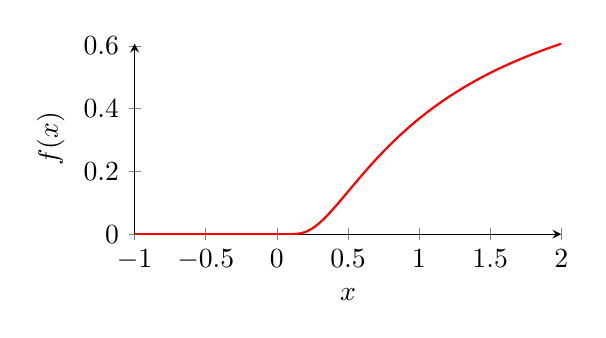
\begin{tikzpicture}
    \begin{axis}[
        axis lines = left,
        xlabel = $x$,
        ylabel = {$f(x)$},
        width=7cm,height=4cm,
    ]
    \addplot [domain=-1:0.01, samples=5, color=red, style={thick}] {0};
    \addplot [domain=0.01:2, samples=50, color=red, style={thick}] {exp(-1/x)};
    \end{axis}
\end{tikzpicture}
\end{minipage}\hfill

Man kann sich leicht davon überzeugen, dass $f$ eine glatte Funktion ist, denn man erhält durch Ableiten jeweils die Negation der Funktion. Falls wir nun die Taylorreihe von $f$ in $0$ entwickeln wollen, dann werden wir die Nullreihe $0+0x+0x^2+... \neq f(x)$ erhalten.
\end{example}
\begin{example}[Binomische Reihe] Die binomische Reihe von \textsc{Newton} ist für $x \in (-1, 1)$ (also auch für irrationale Zahlen!) und $a \in \C$ wie folgt definiert:

$$f_a(x) = \sum_{n=0}^\infty \binom{a}{n} x^n = (1+x)^a$$

\begin{figure}[hbt!]
    \centering
    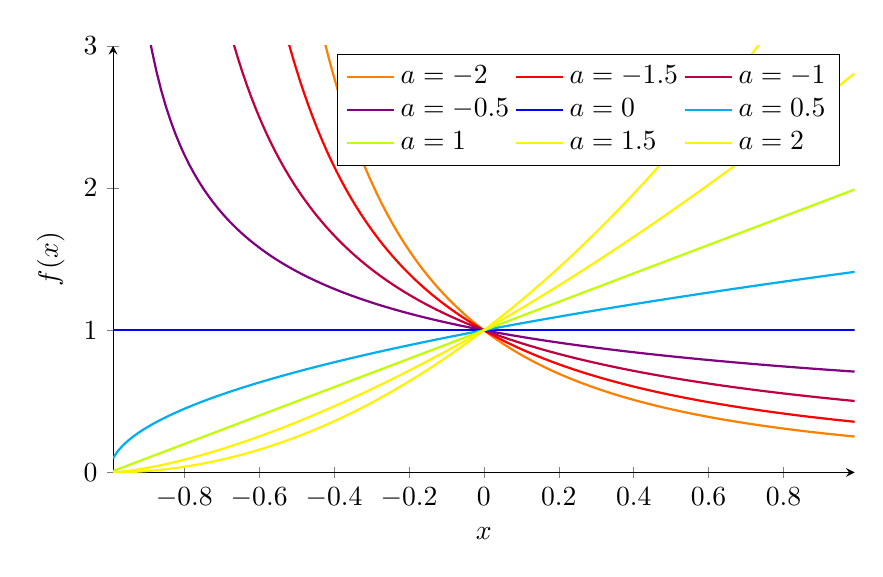
\begin{tikzpicture}
    \begin{axis}[
        axis lines = left,
        xlabel = $x$,
        ylabel = {$f(x)$},
        ymax=3, ymin=-0,
        width=11cm,height=7cm, legend columns=3, 
        legend cell align={left},
    ]
    \addplot [domain=-0.8:0.99, samples=150, style={thick}, color=orange] {(1+x)^(-2)};
    \addlegendentry{$a=-2$}
    \addplot [domain=-0.9:0.99, samples=150, style={thick}, color=red] {(1+x)^(-1.5)};
    \addlegendentry{$a=-1.5$}
    \addplot [domain=-0.9:0.99, samples=150, style={thick}, color=purple] {(1+x)^(-1)};
    \addlegendentry{$a=-1$}
    \addplot [domain=-0.9:0.99, samples=150, style={thick}, color=violet] {(1+x)^(-0.5)};
    \addlegendentry{$a=-0.5$}
    \addplot [domain=-0.99:0.99, samples=150, style={thick}, color=blue] {(1+x)^(0)};
    \addlegendentry{$a=0$}
    \addplot [domain=-0.99:0.99, samples=150, style={thick}, color=cyan] {(1+x)^(0.5)};
    \addlegendentry{$a=0.5$}
    \addplot [domain=-0.99:0.99, samples=150, style={thick}, color=lime] {(1+x)^(1)};
    \addlegendentry{$a=1$}
    \addplot [domain=-0.99:0.99, samples=150, style={thick}, color=yellow] {(1+x)^(1.5)};
    \addlegendentry{$a=1.5$}
    \addplot [domain=-0.99:0.8, samples=150, style={thick}, color=yellow] {(1+x)^(2)};
    \addlegendentry{$a=2$}
    \end{axis}
\end{tikzpicture}
\end{figure}

wobei der \textbf{Binomialkoeffizient} $\binom{a}{n}$ wie folgt definiert ist:
$$\binom{a}{n} = \frac{a(a-1)...(a-n+1)}{n(n-1)...1} = \frac{a!}{n!(a-n)!}$$
Es gilt $\binom{a}{0} = 1$. 

Wir wollen nun also zeigen, dass die explizite Form von $f$ und die Reihe für $f$ äquivalente Formulierungen sind für $f: (-1,1) \to \R$:
\begin{proof}
Zuerst bilden wir die Taylorreihe von der expliziten Form von $f$ um 0 und erhalten:
\begin{align*}
    f(x) &= (1+x)^{a}\\
    f'(x) &= a(1+x)^{a-1}\\
    f''(x) &= a(a-1)(1+x)^{a-2}\\
    &...\\
    f^{(n)}(x)&= a(a-1)(a-2)...(a-n)(1+x)^{a-n}\\
    f^{(n)}(0)&= a(a-1)(a-2)...(a-n+1)\\
    \frac{f^{(n)}(0)}{n!} &= \frac{a(a-1)(a-2)...(a-n+1)}{1\cdot2\cdot...\cdot n} \stackrel{def.}{=} \binom{a}{n}
\end{align*}
für $a\in \C$ und $n \in \N$, wobei $n$ den Index des Gliedes der Taylorreihe bezeichnen soll. Wir müssen nun einige Fallunterscheidungen machen. Betrachten wir zuerst den Fall, in welchem $a \in \N$ gilt. Wir erkennen im Zähler, dass einige Glieder gleich $0$ sein können, nämlich genau die, dessen Index grösser gleich $a$ ist. Des Weiteren wissen wir, dass wegen $n \in N$ für $a \in \C \setminus \N$ jeder Faktor des Zählers ungleich 0 sein muss. Wir erhalten also zusammengefasst:
\begin{align}\label{eq_binomial_cases}
    \binom{a}{n} &= \begin{cases} 0 & , a \in \N, a \leq n \\
    \frac{a!}{n!(a-n)!} & , a \in \N, 0 \leq n < a \\
    \frac{a(a-1)(a-2)...(a-n+1)}{1\cdot2\cdot...\cdot n} & , a \in \C \setminus \N \end{cases}
\end{align}

Wir möchten nun die üblichen zwei Fragen beantworten: 
\begin{enumerate}[label=(\alph*)]
    \item Konvergiert die Taylorreihe von $f$?
    \item Und falls ja, konvergiert sie auch gegen $f$?
\end{enumerate}

Wir zeigen also:

(a) für den Fall $a \notin \N$ mit dem Quotientenkriterium\footnote{Der Quotient von zwei aufeinander folgenden Gliedern konvergiert gegen 0.}:
\begin{align}\label{eq_binomial_identity}
    \frac{\binom{a}{n+1}}{\binom{a}{n}} &= \frac{a(a-1)...(a-n+1)(a-n)}{1\cdot2\cdot...\cdot n \cdot (n+1)} \cdot \frac{1\cdot2\cdot...\cdot \nonumber n}{a(a-1)...(a-n+1)}\\
    &= \frac{a-n}{n+1}
\end{align}
also erhalten wir mit $x$ als Variable:
$$\abs{ \frac{\binom{a}{n+1}x^{n+1}}{\binom{a}{n}x^n}} = \frac{\abs{a-n}}{\abs{n+1}}\abs{x} \xrightarrow{n \to \infty} \abs{x}$$
woraus wir mit dem Quotientenkriterium erkennen, dass die Reihe für $\abs{x} < 1$ konvergiert und für $\abs{x} > 1$ divergiert.

Für den Fall $a \in \N$ bricht die Reihe bei Index $n = a$ ab (siehe \ref{eq_binomial_cases}) und ist somit ein endliches Polynom, welches für alle $x$ konvergiert.

(b) Um die Gleichheit zu zeigen, wollen wir einen gängigen Trick verwenden: Wir wollen zeigen, dass $f$ und die Reihe davon die eindeutige Lösung einer Differentialgleichung mit gegebenen Anfangsbedingungen ist. Unsere Behautung ist also folgende:

(Behauptung) $f(x) = (1+x)^a$ ist die eindeutige Funktion, die
\begin{align*}
    (1+x)f'(x) &= af(x) & x &\in (-1,1)\\
    f(0) &= 1
\end{align*}
erfüllt.

Um diese Behauptung zu beweisen, haben wir zwei Eigenschaften zu zeigen: Die Eindeutigkeit der Funktion, die durch die Einschränkungen der Differentialgleichung gegeben wird und dass die Reihe von $f$ die Differentialgleichung ebenfalls erfüllt:

(Eindeutigkeit) Wir können schnell durch Differenzieren und Einsetzen verifizieren, dass $f$ die Eigenschaften der Behauptung erfüllt. Sei nun $g$ eine weitere Funktion, die $(1+x)g'(x) = a\cdot g(x)$ erfüllt. Wir wollen nun den Quotienten aus $f$ und $g$ bilden und diesen ableiten. Intuitiv sollte klar sein, dass der Quotient konstant sein wird, falls $f$ und $g$ ein Vielfaches voneinander sind. Die Ableitung davon wird also 0 sein:
\begin{align*}
    \frac{d}{dx} \Big(\frac{g(x)}{f(x)}\Big) &= \frac{d}{dx} \big(\frac{g(x)}{(1+x)^a}\big)\\
    &=\frac{g'(x)}{(1+x)^a}-\frac{ag(x)}{(1+x)^{a+1}}\\
    &= \frac{(1+x)g'(x)-ag(x))}{(1+x)^{a+1}} = 0\\
    \implies \frac{g(x)}{f(x)} &= const
\end{align*}
Setzen wir die Anfangsbedingung $g(x) = 1$ ein, so ist die Konstante gleich 1, welches $g(x) = f(x)$ impliziert.

(Reihe erfüllt Bedingungen) Es bleibt zu zeigen, dass $g(x) = \sum_{n=0}^\infty \binom{a}{n} x^n$ die Bedingungen erfüllt:
{\allowdisplaybreaks
\begin{align*}
(1+x) g'(x) &= (1+x) \frac{d}{dx} \Big(\sum_{n=0}^\infty \binom{a}{n} x^n\Big)\\
    &= (1+x) \Big(\sum_{n=1}^\infty \binom{a}{n}n x^{n-1}\Big)\\
    &= \sum_{n=1}^\infty \binom{a}{n}n x^{n-1} + \sum_{n=1}^\infty \binom{a}{n}n x^{n}\\
    &= \sum_{n=0}^\infty \binom{a}{n+1}(n+1) x^{n} + \sum_{n=0}^\infty \binom{a}{n}n x^{n}\\
    &= \sum_{n=0}^\infty \Big( \underbrace{\binom{a}{n+1}}_{(\ref{eq_binomial_identity})}(n+1) + \binom{a}{n}n \Big) x^n\\
    &= \sum_{n=0}^\infty \Big( \binom{a}{n}\frac{a-n}{\cancel{n+1}}\cancel{(n+1)} + \binom{a}{n}n \Big) x^n\\
    &= \sum_{n=0}^\infty \Big( \binom{a}{n} (a-n+n) \Big) x^n\\
    &= \sum_{n=0}^\infty a \binom{a}{n} x^n = a \cdot g(x)
\end{align*}}
Da per Definition $g(0) = \binom{a}{0} = 1$ die Anfangsbedingung erfüllt ist, gilt $g(x) = (1+x)^a$.
\end{proof}
\end{example}
